% Chapter 3
\section*{\centering Preface}
This chapter explains the experimental methods carried out to assemble a battery on a lab-scale. Procedures for preparing cathode slurries and electrolytes for an aluminum-ion cell have been briefly described. 
\pagebreak
\chapter{Experimental methods} % Main chapter title

\label{chap3} % For referencing the chapter elsewhere, use \ref{Chapter1} 

\section{Components of a cathode}
A cathode used in a battery consists of an active material, a binder and a conductive carbon. They are mixed together to form a slurry, which is then coated on to a current collector.  
\begin{itemize}
    \item Active material: The main material that gives a battery its capacity
    \item Binder: A binder is usually a polymer that uniformly binds the cathode materials and allows it to stick firmly on to the current collector. Polytetrafluoroethylene (PTFE or Teflon) and Polyvinylidene fluoride (PVDF) are most commonly used as binders for making battery slurries. It reduces the conductivity of the active  material \cite{grillet_conductivity_2016}. 
    \item Conductive carbon: A conductive form of carbon which is highly amorphous, is added to improve the conductivity of the slurry. Super-P or carbon black or acetylene black is normally used as the conductive agent. 
    \item Current collector: It is typically a metallic foil (copper, aluminium, steel, etc.) onto which the slurry is coated. The main role of the current collector is to support the electrode material and to collect the accumulated electrical energy from the electrode and then allow the current to flow into the external circuit\cite{sun_effect_2017}.
\end{itemize}

\section{Formation of slurry}
A slurry is a paste-like substance used in making battery electrodes. It is important for slurries to be homogeneous. This helps in getting a uniform coating at later stages. To make a slurry, the binder, PVDF was mixed separately in an organic solvent, N-methyl pyrrolidinone (NMP). The viscous solution was added to a separate mixture of active material and Super-P. NMP can be added at any given time to adjust the consistency of the slurry. It was then mixed on a magnetic stirrer for 8-10 hours. 

\section{Preparing a cathode}
Once the slurry was prepared, it was 'doctor-bladed' on a current collector. Doctor blading is a coating process where the slurry spreads on a substrate (molybdenum foil)  using a blade, to form a thin sheet which dries off to give a layer of coating.  Initially, nickel (Ni) foils were used as current collectors. However it was found that the Ni oxidised at $\sim$ 1.0 V. This did not allow the cell to reach it's cut-off voltage at 2.4 V. It impeded the cell's redox processes, which reduced the cell's capacity. After trying a few current collectors (discussed in Chapter \ref{chap7}), it was found that molybdenum foil did not contribute any capacity of its own and was completely inert during the entire process (discussed in Appendix A). Thus, it was used in all our battery systems. After coating the foils with the slurry, the electrodes were dried at 80$^{\circ}$C for two hours to improve the adhesion of the slurry onto the Mo foil. 

\begin{figure}[tbh!]
\centering
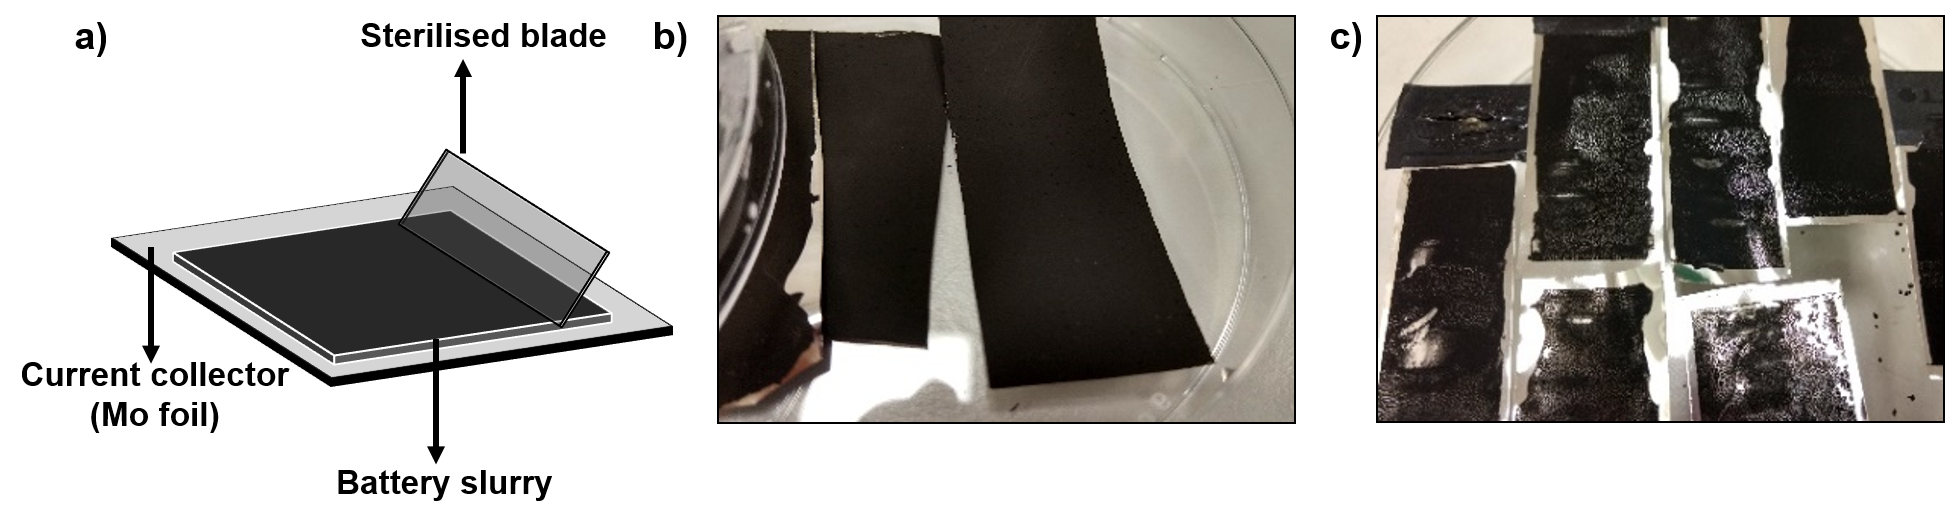
\includegraphics[width=\textwidth]{Figures/chap3fig/coating}
\caption{a) Doctor-blading on a current foil using a steel blade. A dried cathode after b) uniform and c) non-uniform coating.}
\label{Figures/chap3fig:coating}
\end{figure}

\section{Vacuum drying}
The cathodes were then vacuum dried at 120$^{\circ}$C for 12 hours. Vacuum drying is a moisture-removal technique by means of creating a vacuum. It is used for drying things which are hygroscopic (water sensitive). In this case, vacuum was created, which decreased the chamber pressure below vapor pressure of the solvent (NMP), causing it to boil. This increases its rate of evaporation and also the drying rate of the product. The cathodes are ready for use after drying. 

\section{Assembling a cell}

\subsection*{Coin cells}
Using pouch cells or coin cells (CR-2032\textregistered) is a common practice amongst researchers who work on batteries. CR-2032, a type of coin cell, is made of steel and was used for making cells, shown in Figure \ref{Figures/chap3fig:concell}a. However, the \ce{AlCl3}/EMImCl electrolyte reacted with the chromium in steel and resulted in corrosion of the battery parts (Figure \ref{Figures/chap3fig:concell}b) \cite{das_aluminium-ion_2017}. The cells as a result short circuited and produced expendable results displayed in Figure \ref{Figures/chap3fig:weirdcdc}a and b. VUW lacked the facilities to produce pouch cells (more efficient battery design). To overcome all the above-mentioned problems, Swagelok-type cells were designed at VUW and used. The custom-made cell is illustrated in Figure \ref{Figures/chap3fig:swagelok}a. PEEK (polyether ether ketone) was used for the main body and metal rods were used as plungers. Their role was to push the electrodes towards each other. PEEK is a colourless organic thermoplastic polymer. It has a melting point of 343$^{\circ}$C, with excellent mechanical and chemical resistance properties. Molybdenum (Mo) rods were chosen as metal plungers instead of steel, which is generally used in Swagelok-type cells because of the aforementioned corrosion issues. 

\begin{figure}[tbh!]
\centering
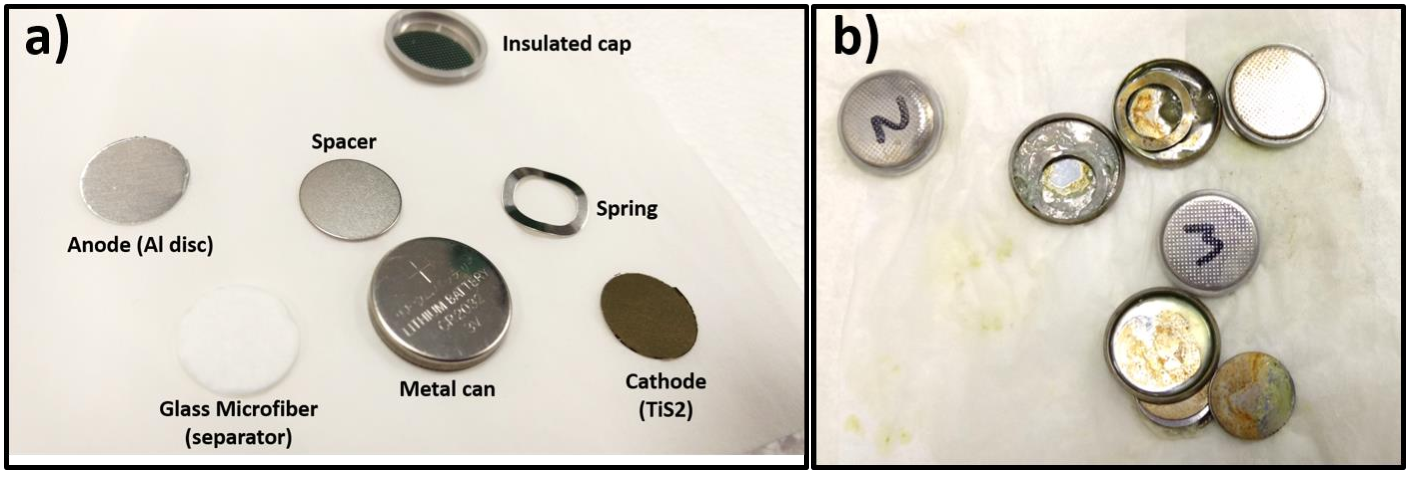
\includegraphics[width=\textwidth]{Figures/chap3fig/concell.pdf}
\caption{Components of a coin cell. The metallic can, spacers and the spring is made of steel.}
\label{Figures/chap3fig:concell}
\end{figure}

\begin{figure}[tbh!]
\centering
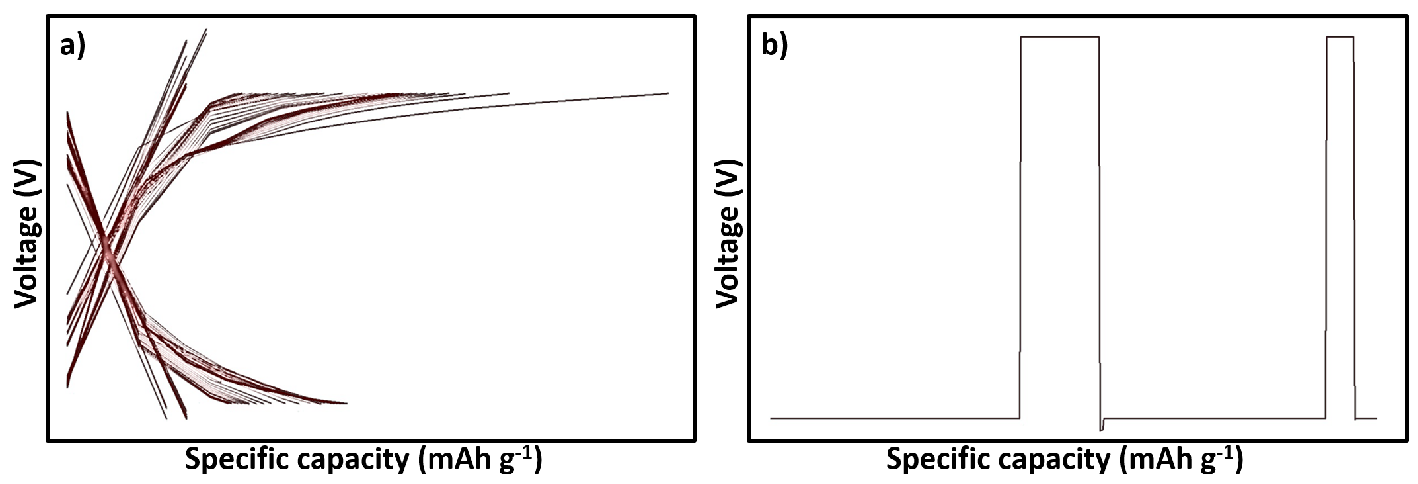
\includegraphics[width=\textwidth]{Figures/chap3fig/weirdcdc}
\caption{Examples of unexpected charge/discharge curves using a coin cell. The data obtained from both these graphs indicated short circuits and/or some parasitic reactions. a) Specific capacities as low as 0.05 mAh g$^{-1}$ were recorded at lower current rate (10 mA g$^{-1}$) which were meaningless. b) A short circuit or a wrong battery connection in the cell yielded a chronopotentiogram (voltage vs. time plot) with rectangular blocks.}
\label{Figures/chap3fig:weirdcdc}
\end{figure}

\begin{figure}[tbh!]
\centering
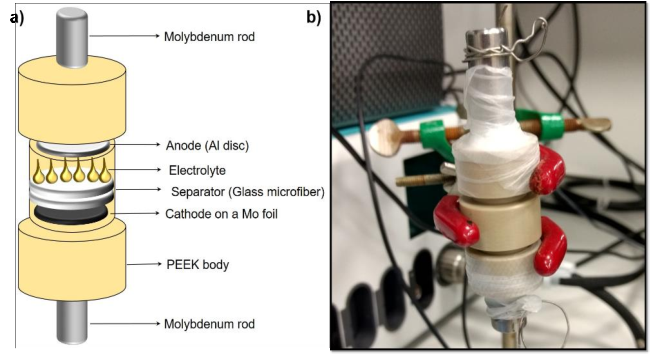
\includegraphics[width=\textwidth]{Figures/chap3fig/swagelok.pdf}
\caption{a) Assembling a two-electrode PEEK cell using a cathode, separators wetted with electrolyte and an anode. Mo rods were used as plungers and Mo sheets was used as current collector. b) A custom-made lab cell ready for preliminary electrochemical measurements.}
\label{Figures/chap3fig:swagelok}
\end{figure}

\subsection*{Cell assembly}
A cathode was placed at the bottom of the cell, two separators made of glass microfibers were placed above the cathode. Electrolyte was added ($\sim$80 $\mu$l) until the separators were completely wet. An anode, 99\% pure aluminium foil, was cut into a disc and placed on top and the cell was then screwed tight, shown in Figure \ref{Figures/chap3fig:swagelok}a. Since the electrolyte is hygroscopic, the cell was assembled inside a glove box with <0.1ppm \ce{O2}/\ce{H2O}. The cell was taken out of the glove box and wrapped tightly with a paraffin film to inhibit any further contact with moisture or air, as shown in Figure \ref{Figures/chap3fig:swagelok}b. The cell was then ready for electrochemical measurements . 

\subsection*{Choosing the right instrument}
To measure battery capacity, an instrument is needed that controls the potential difference between two electrodes: working electrode (WE) and reference electrode(RE) in an electrochemical cell. A working electrode is where the current is measured and provides a surface on which electrochemical reactions take place. A two-electrode setup was used for all electrochemical analysis i.e. charge/discharge cycles and cyclic voltammetry. The WE was attached to the cathode side and CE and RE are connected to the anode side of the PEEK cell. To measure the specific capacities at constant current rates, a galvanostat was used. Interestingly, a potentiostat can also act as a galvanostat if the received feedback is switched from the cell voltage signal to the cell current signal. The instrument then controls the cell current rather than the cell voltage. \\
For measuring the charge/discharge cycles, PGSTAT-128N, a potentiostat from \textit{Metrohm, Autolab} was used, which was turned into a galvanostat. Unfortunately, the galvanostat only had one channel, which meant only one cell could be measured at a given time. The instrument was highly sensitive and susceptible to noise pick-up. Analysing data was next to impossible since the software crashed, after two or three cycles. \\
To prevent this, \textit{Neware} BTS-4000, a battery analyser was ordered from China. A battery analyser is a cheaper and a simpler version of the galvanostat. It is easier to handle and has a number of ports available for cell analysis, which allows an independent channel control. The data acquisition frequency was 1 data point for every 0.01 second. This instrument stored data from thousands of cycles, which was not possible from a single-channel potentiostat. 

\subsection*{Protocol optimisation}
Testing a battery involves a wide range of tests to analyse both the chemical and physical properties of the material used. It is also important to evaluate their electrical, mechanical, and life time performance under different environmental conditions.
Carrying out these tests needed a well equipped test facility, with the ability to cycle cells through repetitive charge/discharge cycles. Finding the correct instrument for electrochemical analyses, setting them up and establishing a standard protocol took significant amount of time in the first few months of this project. Developing a standard protocol for charge/discharge cycles was an important milestone. A number of attempts were made to finalise a standard testing protocol. It was observed that a very high or a very low current rate was detrimental to the cell (discussed on page 7). The cells were usually discharged or charged at 50 or 100 mA g$^{-1}$, for 50 cycles, at room temperature. The potential window for these cycles was 0.02 V to 2.35 V. 
The standardised protocol for a continuous charge/ discharge cycles is illustrated in Figure \ref{Figures/chap3fig:flow}

\begin{figure}[tbh!]
\centering
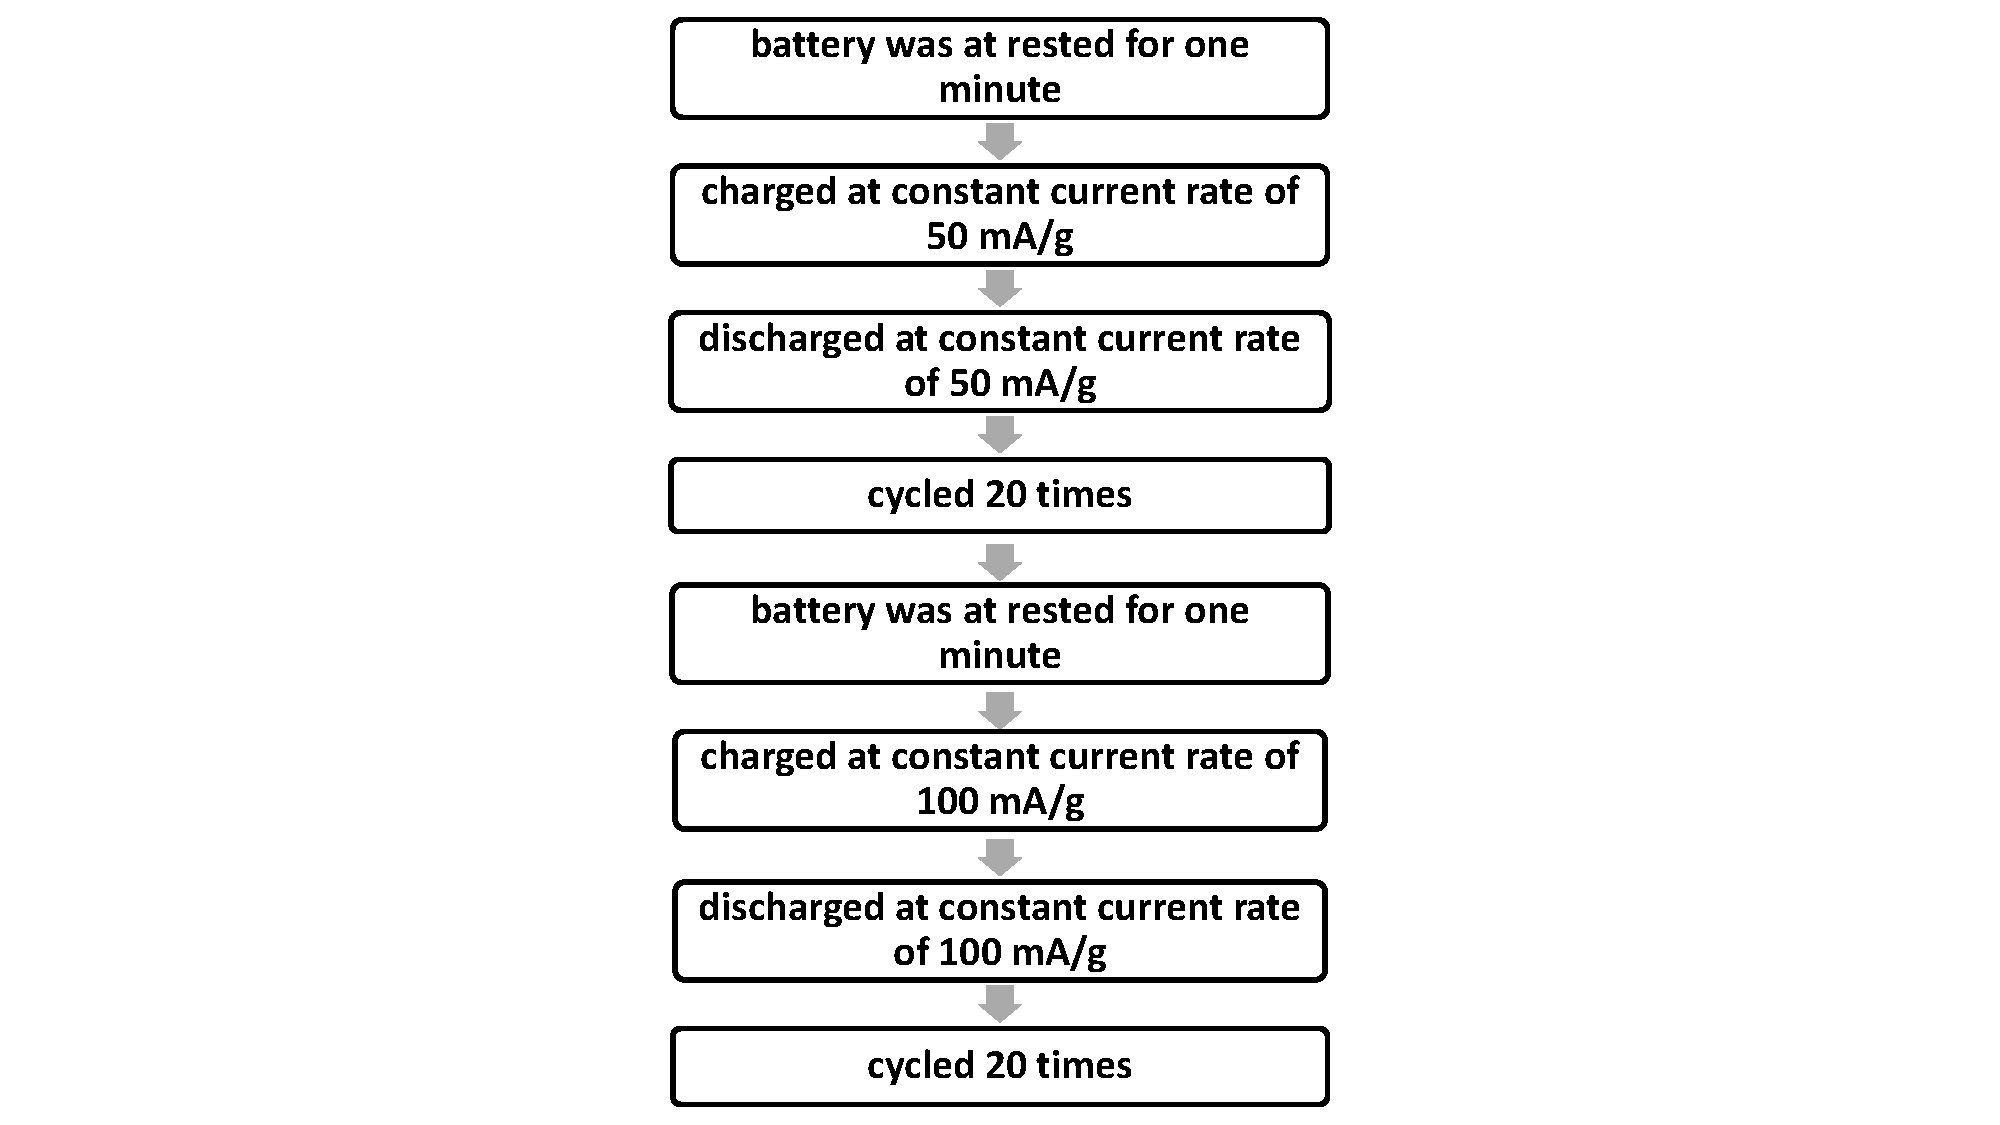
\includegraphics[width=\textwidth]{Figures/chap3fig/flow.pdf}
\caption{A flow chart illustrating the standard protocol for battery testing. This protocol was finalised after a number of failed attempts.}
\label{Figures/chap3fig:flow}
\end{figure}

Similar procedure was followed at current rates varying from 50-1500 mA g$^{-1}$.\\
The ability of the battery to accept very high currents is determined by the following factors:
\begin{itemize}
    \item high surface area electrodes
    \item low volume change during ion-insertion to avoid mechanical stress on the crystal structures
    \item low internal impedance to minimise the energy loss and heat generation in the cell
\end{itemize}

High rate performance is a prerequisite for both high energy density and fast charging. High capacity batteries use very high charge rates in order to achieve reasonable charging times. However, since this project required a comprehensive analysis and most of them were new materials, lower charge/discharge rates were used. 
The major challenge in the search for the optimum cell chemistry is that all the above-mentioned performance parameters are inter-related. Improving one of these parameters can adversely affect the performance of one or more of the others. To verify the cell performance every time a change is made, repetitive testing, particularly lifetime testing is required, which can take many years.





















